\begin{frame}{Três configurações do filtro RC}
  \begin{columns}[T,onlytextwidth]
    \begin{column}{0.31\textwidth}
      \centering
      \textbf{1. Sem carga}

      \vspace{0.16cm}
      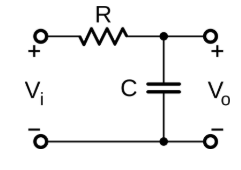
\includegraphics[width=\linewidth,height=0.31\textheight,keepaspectratio]{slides/img/circuito_1.png}

      \begin{block}{Referência}
        \small Saída medida sobre o capacitor, sem uma carga resistiva adicional.
      \end{block}
    \end{column}
    \begin{column}{0.31\textwidth}
      \centering
      \textbf{2. Com carga direta}

      \vspace{0.16cm}
      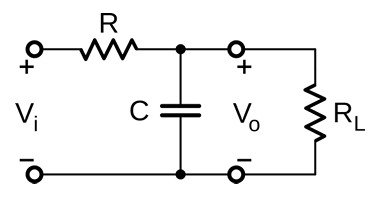
\includegraphics[width=\linewidth,height=0.31\textheight,keepaspectratio]{slides/img/circuito_2.png}

      \begin{block}{Efeito de carga}
        \small $R_L$ fica em paralelo com $C$, alterando o ganho e a constante de tempo.
      \end{block}
    \end{column}
    \begin{column}{0.31\textwidth}
      \centering
      \textbf{3. Com buffer}

      \vspace{0.16cm}
      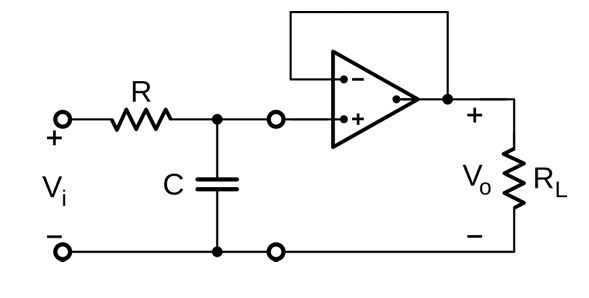
\includegraphics[width=\linewidth,height=0.31\textheight,keepaspectratio]{slides/img/circuito_3.png}

      \begin{block}{Isolamento}
        \small O seguidor de tensão fornece corrente à carga sem carregar o nó RC ideal.
      \end{block}
    \end{column}
  \end{columns}
\end{frame}
